\newpage
%Kapitelüberschrift
\section{Architektur}
\subsection{Auswahl der Architektur}
Die Architektur wurde stark dem Yolo-Paper \cite{yolo} angelehnt. 
Dies obwohl zu diesem Zeitpunkt auch schon das Yolo v2-Paper \cite{yolo2} erschienen war.
Es gab damals schon viele gute Gründe dafür von Beginn weg das Netzwerk und Kostenfunktionen nach dem Yolo v2-Paper aufzubauen.
So ist Yolo v2 nach dessen Paper zu urteilen schneller und genauer. 
Der Grund, warum trotzdem Yolo v1 verwendet wurde, war dass die Beschreibung z.B. von Kostenfunktion und von der Architektur im Paper von Yolo v1 um einiges genauer und verständlicher war als im Paper von Yolo v2.
Ausserdem ging man mit der Einstellung an die Arbeit, dass wenn erst das \grqq{}einfache\grqq{} Yolo v1  erfolgreich implementiert wurde, dieses entsprechend immer noch zur 2. Version erweitert werden könnte.

\todo[inline,size=\Large]{evtl. den folgenden Abschnitt entfernen.}

Dazu kam es allerdings nicht, weil verschiedene Faktoren die erfolgreiche Fertigstellung von v1 verzögerten. 
(Genauere Informationen dazu werden später im Kapitel \todo[inline,size=\Large]{min. hier eine Referenz auf die Erklärung warum die Verzögerungen auftraten machen.} erläutert.) 
Ausserdem war das Grundlegende Ziel immer einen Eindruck dafür zu bekommen, was mit State-Of-The-Art Lösungen aktuell in diesem Bereich überhaupt möglich wäre.
Entsprechend hatte man sich auch primär auf dieses Ziel fokussiert.

\subsection{Architekturaufbau}
\label{chapter:Architekturaubau}
\subsubsection{Hauptgraph}

\begin{table}
\centering
\begin{tabularx}{1.1\textwidth}{|l|l|l|l|l|X|}
\hline
\textbf{Layer} & \textbf{Filtertyp}  & \textbf{Anzahl} & \textbf{Grösse} & \textbf{Strides} & \textbf{Output} \\
\hline 	0	& Input				&		&		&		& 448x448x1\\
\hline 	1	& Convolutional		& 64		& 7x7	& 2x2	& 224x224x64	\\
\hline 	2	& Maxpool      		& 		& 2x2	& 2x2	& 112x112x64	\\
\hline 	3   & Convolutional		& 192	& 3x3	& 1x1	& 112x112x192\\
\hline 	4	& Maxpool			& 		& 2x2	& 2x2	& 56x56x192	\\
\hline 	5	& Convolutional		& 128	& 1x1	& 1x1	& 56x56x128	\\
\hline 	6	& Convolutional		& 256	& 3x3	& 1x1	& 56x56x256	\\
\hline 	7	& Convolutional		& 256	& 1x1	& 1x1	& 56x56x256	\\
\hline 	8	& Convolutional		& 512	& 3x3	& 1x1	& 56x56x512	\\
\hline 	9	& Maxpool			&		& 2x2	& 2x2	& 28x28x512	\\
\hline 	10	& Convolutional		& 256	& 1x1	& 1x1	& 28x28x256	\\
\hline 	11	& Convolutional		& 512	& 3x3	& 1x1	& 28x28x512	\\
\hline 	12	& Convolutional		& 256	& 1x1	& 1x1	& 28x28x256	\\
\hline 	13	& Convolutional		& 512	& 3x3	& 1x1	& 28x28x512	\\
\hline 	14	& Convolutional		& 256	& 1x1	& 1x1	& 28x28x256	\\
\hline 	15	& Convolutional		& 512	& 3x3	& 1x1	& 28x28x512	\\
\hline  	16	& Convolutional		& 256	& 1x1	& 1x1	& 28x28x256	\\
\hline  	17	& Convolutional		& 512	& 3x3	& 1x1	& 28x28x512	\\
\hline 	18	& Convolutional		& 512	& 1x1	& 1x1	& 28x28x512	\\
\hline  	19	& Convolutional		& 1024	& 3x3	& 1x1	& 28x28x1024	\\
\hline  	20	& Maxpool			&		& 2x2	& 2x2	& 14x14x1024	\\
\hline  	21	& Convolutional		& 512	& 1x1	& 1x1	& 14x14x512	\\
\hline  	22	& Convolutional		& 1024	& 3x3	& 1x1	& 14x14x1024	\\
\hline  	23	& Convolutional		& 512	& 1x1	& 1x1	& 14x14x512	\\
\hline  	24	& Convolutional		& 1024	& 3x3	& 1x1	& 14x14x1024	\\
\hline  	25	& Convolutional		& 1024	& 3x3	& 1x1	& 14x14x1024	\\
\hline  	26	& Convolutional		& 1024	& 3x3	& 2x2	& 7x7x1024	\\
\hline  	27	& Convolutional		& 1024	& 3x3	& 1x1	& 7x7x1024	\\
\hline  	28	& Convolutional		& 1024	& 3x3	& 1x1	& 7x7x1024	\\
\hline 	31	& Fully-Connected	&		&(7x7x1024)x4096	&	& 4096  \\
\hline  	32	& Fully-Connected	&		& 4096x(7x7x6)	&	& 7x7x6 \\
\hline 	
\end{tabularx}
\caption{Yolo-Architektur}
\label{tbl:yolo_architektur}
\end{table}


Der grundlegende Aufbau der Architektur, wie er letztendlich aussah kann man in der Tabelle \ref{tbl:yolo_architektur} betrachten. 
Dies sah allerdings noch nicht immer so aus.
Obwohl die Convolution-Filter schon immer so ausgesehen hatten, sah der ursprüngliche Bildinput und entsprechend die Outputs der verschiedenen Layers mal anders aus.
Nach ausführlicher Diskussion \cite{PrivateCommunication} wurde zu Beginn des Architekturdesigns entschieden, dass man nicht mit 448x448 Bildern arbeitet, wie dies im Yolo-Paper \cite{yolo} gemacht wurde.
Der Grund dafür war, dass für das Training wie auch später für den Praxiseinsatz immer 1280x960 grosse Bilder zur Verfügung standen und man entsprechend nicht Informationen \grqq{}wegwerfen\grqq{} sondern so lange wie möglich im Netz behalten wollte.
So war der Input (Layer 0 in Tabelle \ref{tbl:yolo_architektur}) damals 1280x960x1, entsprechend dann auch der Output von Layer 1 nicht mehr 224x224x64 sondern 640x480x64 usw.
Da dies am Schluss nicht aufgeht mit dem Netzwerk, hatte es damals noch zwei zusätzliche Layer (29 \& 30), welche jetzt nicht mehr vorhanden sind.
Layer 29 war dabei für ein Zeropadding und Layer 30 für ein Maxpooling mit Strides 3x3 zuständig.


\begin{figure}
	\centering
	\begin{minipage}[b]{0.48\textwidth}	
		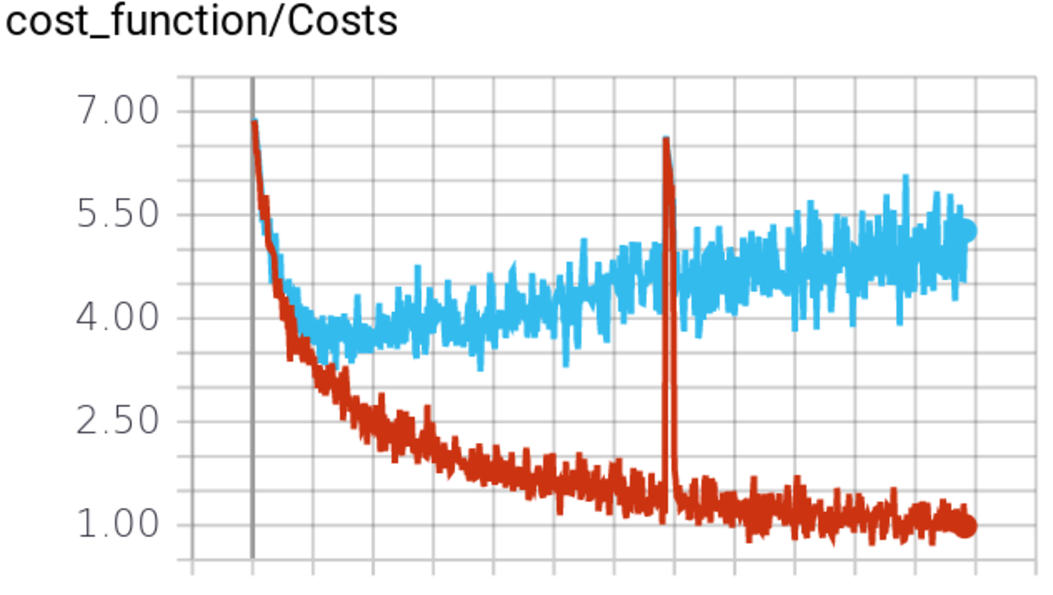
\includegraphics[width=\textwidth]{Kapitel/40Architektur/Bilder/OverflowInPretraining.pdf}
	\end{minipage}
	\hfill
	\begin{minipage}[b]{0.48\textwidth}		
		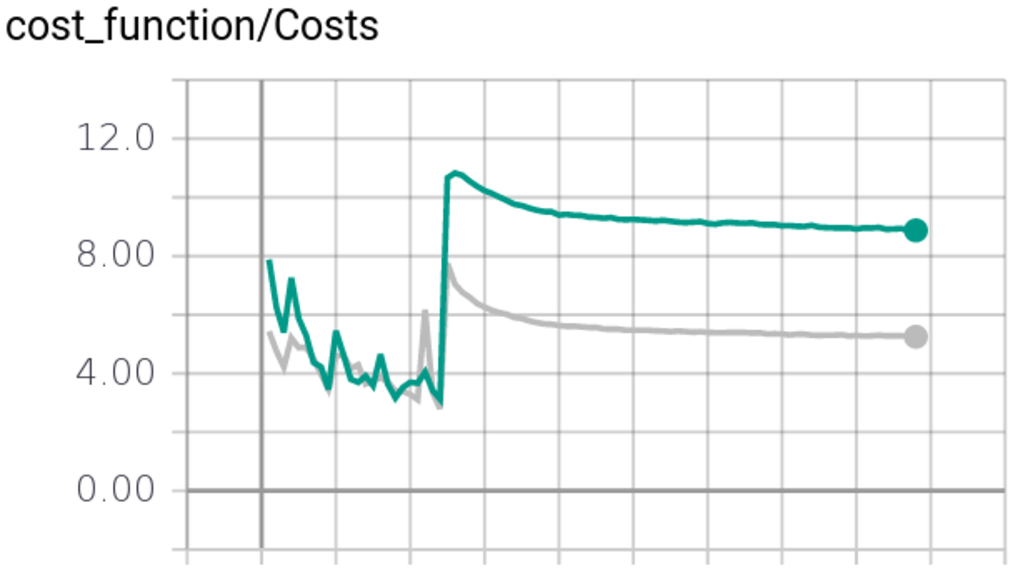
\includegraphics[width=\textwidth]{Kapitel/40Architektur/Bilder/OverflowInTraining.pdf}
	\end{minipage}
			\caption{Effekte (Extremer Anstieg der Kosten innert einer Epoche) im Pretraining(links) und im Training(rechts). x-Achse=Zeit, y-Achse=Kosten. Weinrot=Pretraining-Trainingsdaten, Hellblau=Pretraining-Validierungsdaten, Grün=Training-Trainingsdaten, Grau=Training-Validierungsdaten}
	\label{img:Overflow}
\end{figure}



Diese damalige Architektur war zu gross, um sie auch nur mit Minibatchsize=1 und Float32 ins GPU-RAM und entsprechend überhaupt zum laufen zu kriegen. 
Entsprechend wurden alle Gewichte und Knoten mit Float16 initialisiert. 
Seit dieser Initialisierung war eine Minibatchsize=7 möglich.

Mit dieser Architektur wurde eine Zeit lang trainiert, bis sich immer mehr spezielle Effekte im Training, wie auch im Pretraining (Details zum Pretraining im Kapitel \ref{chapter:Pretraining}) häuften.
Es konnte auch nach längerer Analyse nicht abschliessend geklärt werden, was die Ursache für diese Effekte (Siehe Abbildung \ref{img:Overflow}) war.
Die Vermutung lag jedoch darin, dass es sich um Overflow-Probleme im Zusammenhang mit den verwendeten Float16 handeln könnte.
Entsprechend wurde die Architektur umgebaut, sodass die Input-Bilder künstlich verkleinert wurden, um dafür Float32 verwenden zu können.
In diesem Schritt war es naheliegend, dass man sich gleich den originalen Werten, wie sie von Yolo \cite{yolo} verwendet wurden annäherte.
Entsprechend wurden die Input-Bilder auf 448x448 verkleinert.
Dies hatte wiederum zur Folge, dass seit diesem Zeitpunkt sogar eine Minibatchsize=24 verwendet werden konnte.
Ausserdem, und dies war noch viel wichtiger, traten die genannten speziellen Effekte (Abbildung \ref{img:Overflow}) weder im Pretraining noch im Training je wieder auf. 

\begin{table}
\centering
\begin{tabularx}{\textwidth}{|X|l|l|l|}
\hline  Beschreibung & Anzahl & in Bytes(Float16) & in Bytes(Float32)\\
\hline  Gewichte											& 206 M 	& 413 MB 	& 827 MB		\\
\hline  Knoten:Input=1280x960 							&  98 M 	& 186 MB 	&			\\
\hline  Knoten:Input=1280x960 Minibatchsize=7, GPU-RAM voll	& 689 M 	& 1.38 GB 	& 			\\
\hline  Knoten:Input=448x448 							&  16 M 	& 			& 64M 		\\
\hline  Knoten:Input=448x448, Minibatchsize=24, GPU-RAM voll	& 384 M 	& 			& 1.54GB 	\\
\hline
\end{tabularx}
\caption{Anzahl Gewichte und Knoten}
\label{tbl:anzahl_gewichte_knoten}
\end{table} 

Aus dieser Erfahrung kann man ableiten, dass bei Convolutional-Neural-Networks die Grösse der Input-Bilder mehr ins Gewicht fallen als die Anzahl Gewichte. 
Dies scheint nachträglich auch logisch, denn die Bilder werden während dem \grqq{}flow\grqq{} durch das Netzwerk mehrmals zwischengespeichert.
In der Tabelle \ref{tbl:anzahl_gewichte_knoten} ist die Berechnung, der Anzahl Gewichte und der Anzahl Knoten unter der Annahme, dass jedes Bild zwischen den Layern einmal als Knoten abgespeichert wird.
Dabei wurde nicht berücksichtigt, dass es pro Layer mehrere Einheiten von Knoten geben kann, wie z.B. vor und nach der Aktivierungsfunktion. 
Auch ohne diese zusätzlichen Layer kann man aber deutlich erkennen, dass wenn man die Minibatchsize solange erhöht, bis das GPU-RAM (im Rahmen dieser Arbeit 16GB) voll ist, man klar mehr Speicher für Knoten benötigt, als für Gewichte.

\subsubsection{Minibatchnorm}
Zu Beginn des Trainings gab es immer wieder das Problem von vanishing Gradients (Die Gradienten wurden im Verlauf der Backpropagation immer kleiner, bis sie nur noch gleich Null waren.).
Um diesem Problem entgegenzuwirken wurde die relativ junge Allzweckwaffe der Minibatch normalisierung angewandt.
Dabei wird in jedem Convolutional Layer direkt nach dem Convolutional filter der Ausgang über den ganzen Minibatch normiert.
Es wurde auch ausprobiert die Minibatchnorm nach der Relu einzusetzen, anstelle davor, allerdings waren die Ergebnisse der Kostenfunktion bei der Anordnung in Abbildung \ref{img:Conv-Layer} ganz leicht besser.
Die Verbesserung war allerdings nur sehr marginal, weshalb sie auch gerade so gut zufällig sein konnte.
Seit dem Einsetzen der Minibatchnorm war das Netzwerk hervorragend in der Lage die Gradienten per Backpropagation bis zum Eingang des Netzwerks zurück zu tragen. 

\subsubsection{Aktivierungsfunktion}
\begin{figure}
	\centering	
	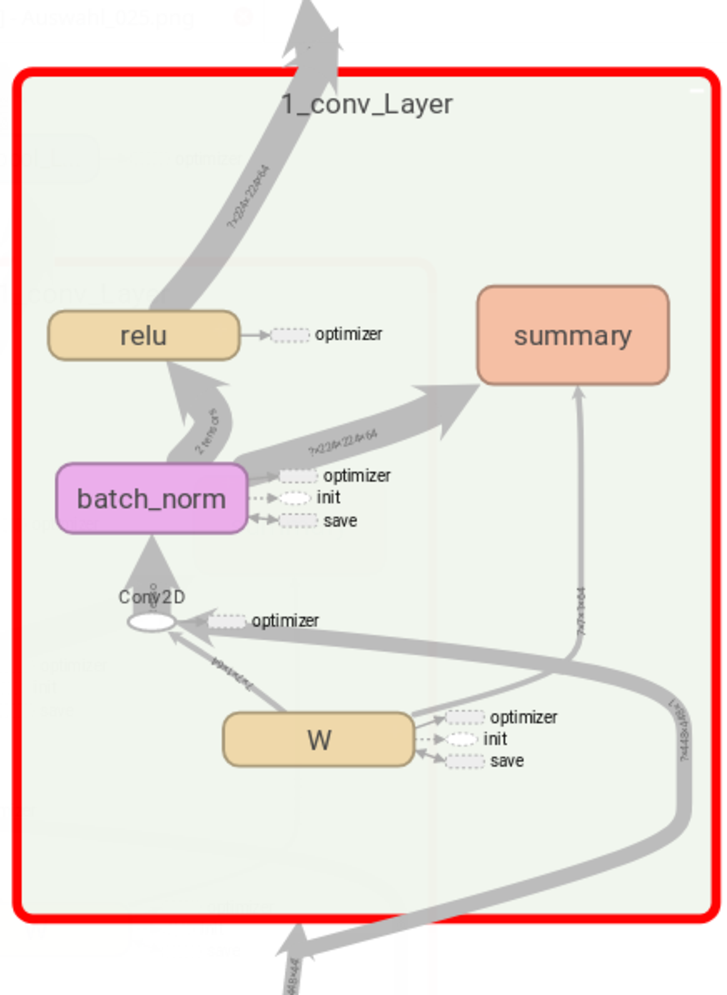
\includegraphics[width=0.5\textwidth]{Kapitel/40Architektur/Bilder/GraphProLayer.pdf}
	\caption{Aufbau eines Convolutional-Layers}
	\label{img:Conv-Layer}
\end{figure}

Wie in Abbildung \ref{img:Conv-Layer} ersichtlich wurde als Aktivierungsfunktion eine simple Relu (Rectified Linear Unit) verwendet. Dies obwohl in yolo v1 eine leaky Relu verwendet wurde.
Der Grund für diesen Wandel war, dass seit dem verwenden der Minibatchnorm eine leaky Relu dieselbe Performance an den Tag legte wie eine normale Relu.

\subsubsection{Dropout}
Es wurde im Rahmen dieser Arbeit viel mit Dropout Experimentiert.
So wurde Dropout in allen, nur in den letzten, nur in den fully-connected Layer oder auch in gar keinem Layer angewandt.
Die besten Performance wurden erreicht, wenn entweder nur in den letzten paar Layern oder auch nur in den fully-connected Layern Dropout eingesetzt wurde.
Wurde Dropout in allen Layern angewandt, war das Resultat massiv schlechter.

Wichtig zu wissen: Wenn man Dropout in Convolutional Layern anwendet, sollte darauf geachtet werden, dass man nicht einzelne Knoten von Dropout \grqq{}ausknippsen\grqq{} lässt, sondern gleich ganze Featuremaps.
Der Grund dafür liegt darin, dass man mit der ursprünglichen Philosophie von dropout eigentlich Gewichte zwischenzeitlich ausschaltet.
Bei Fullyconnected Netzwerken ist dies problemlos möglich, indem man einfach Knoten zufällig auf Null setzt. 
In Convolutional Neural Networks hingegen werden die Gewichte nicht ausgeschaltet, indem man einen Knoten ausschaltet.
Dies, weil die Gewichte über die Bilder oder Feature-Maps geschoben werden und nicht einzelnen Knoten zugeteilt sind.


\subsection{Fazit}
Was die Architektur angeht kann man aus dieser Arbeit die folgenden beiden Punkte lernen:
\begin{enumerate}
\item Wenn in Convolutional Neural Networks Speicherknappheit ein Problem ist, sollte entweder die Tiefe des Netzwerks verkleinert (weniger Layer = weniger Knoten) oder der Input verkleinert (= ebenfalls weniger Knoten) werden. Nicht aber sollte man auf Bastellösungen ausweichen, sodass man sich was Datentypen angeht ausserhalb des Tensorflow-Standardbereichs aufhält. Es sei denn natürlich, man weiss ganz genau was man tut, und kennt entsprechend den Source-Code von Tensorflow in- und auswendig. Wenn dem aber so wäre, würden Sie diese Arbeit wohl kaum lesen ;) .
\item Wenn man eine Architektur nach entsprechend einer Vorlage aufbaut, sollte man nicht schon bevor man eine erfolgreich lauffähige Version hat an Parametern wie der Input-Grösse herumoptimieren. Optimieren sollte man erst, wenn man eine Lauffähige Fehlerfreie Version hat, sodass man jederzeit wieder zu dieser Lauffähigen Version zurückkehren kann.
\item Es trat zu Beginn des Trainings öfters das Problem auf, dass das Programm abstürzte.
Dabei war die Fehlermeldung jeweils, dass NAN (Not a Number) oder Infinity ins Tensorboard gespeichert werden sollte.
Seit die Gradienten auf die Zahl 5/-5 begrenzt wurden, trat dieses Problem auch nie mehr auf.
Daraus folgt: Gradient Clipping ist nur zu empfehlen, da es nicht schadet aber auf jeden Fall allfällige Probleme fernhalten kann. 
\end{enumerate}




